\chapter{Interference solution}
\begin{abox}
	Practice set 1 solutions
	\end{abox}
\begin{enumerate}
\begin{minipage}{\textwidth}
	\item In a Young's double slit interference experiment, the slits are at a distance $2 L$ from each other and the screen is at a distance $D$ from the slits. If a glass slab of refractive index $\mu$ and thickness $d$ is placed in the path of one of the beams, the minimum value of $d$ for the central fringe to be dark is
	\exyear{NET DEC 2011}
\end{minipage}
\begin{tasks}(2)
	\task[\textbf{A.}] $\frac{\lambda D}{(\mu-1) \sqrt{D^{2}+L^{2}}}$
	\task[\textbf{B.}] $\frac{\lambda D}{(\mu-1) L}$
	\task[\textbf{C.}]$\frac{\lambda}{(\mu-1)}$
	\task[\textbf{D.}]$\frac{\lambda}{2(\mu-1)}$
\end{tasks}
\begin{answer}
	$$\text { For central fringe to be dark, }(\mu-1) d=\frac{n \lambda}{2} \Rightarrow d=\frac{\lambda}{2(\mu-1)}$$
	The correct option is \textbf{(d)}	
\end{answer}
\begin{minipage}{\textwidth}
	\item Consider the interference of two coherent electromagnetic waves whose electric field vectors are given by $\vec{E}_{1}=\hat{i} E_{0} \cos \omega t$ and $\vec{E}_{2}=\hat{j} E_{0} \cos (\omega t+\varphi)$ where $\varphi$ is the phase difference. The intensity of the resulting wave is given by $\frac{\varepsilon_{0}}{2}\left\langle E^{2}\right\rangle$, where $\left\langle E^{2}\right\rangle$ is the time average of $E^{2}$. The total intensity is
	\exyear{NET JUNE 2012}
\end{minipage}
\begin{tasks}(2)
	\task[\textbf{A.}] 0
	\task[\textbf{B.}]$\varepsilon_{0} E_{0}^{2}$
	\task[\textbf{C.}] $\varepsilon_{0} E_{0}^{2} \sin ^{2} \varphi$
	\task[\textbf{D.}] $\varepsilon_{0} E_{0}^{2} \cos ^{2} \varphi$
\end{tasks}
\begin{answer}
	Since waves are polarized in perpendicular direction hence there will be no interference.\\
	The correct option is \textbf{(a)}	
\end{answer}
\begin{minipage}{\textwidth}
	\item A parallel beam of light of wavelength $\lambda$ is incident normally on a thin polymer film with air on both sides. If the film has a refractive index $n>1$, then second-order bright fringes can be observed in reflection when the thickness of the film is
	\exyear{NET DEC 2014}
\end{minipage}
\begin{tasks}(2)
	\task[\textbf{A.}] $\lambda / 4 n$
	\task[\textbf{B.}]$\lambda / 2 n$
	\task[\textbf{C.}]$3 \lambda / 4 n$
	\task[\textbf{D.}] $\lambda / n$
\end{tasks}
\begin{answer}
	For constructive interference: $2 n d \cos \theta=(2 m+1) \frac{\lambda}{2}$\\
	For normal incidence $(\theta=0)$ and second $\operatorname{order}(m=1)$ $\Rightarrow 2 n d \cos 0=(2 \times 1+1) \frac{\lambda}{2} \Rightarrow d=\frac{3 \lambda}{4 n}$\\
	The correct option is \textbf{(c)}	
\end{answer}
\begin{minipage}{\textwidth}
	\item A screen has two slits, each of width $w$ with their centres at a distance $2 w$ apart. It is illuminated by a monochromatic plane wave travelling along the $x$-axis.
	The intensity of the interference pattern, measured on a distant screen, at an angle
	$\theta=\frac{n \lambda}{w} \text { to the } x \text {-axis is }$
	\exyear{NET DEC 2016}
	\begin{figure}[H]
		\centering
		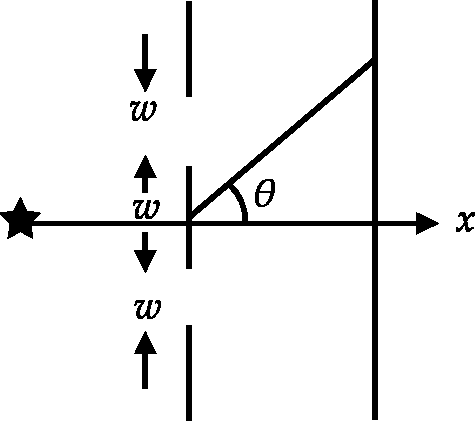
\includegraphics[height=4cm,width=5cm]{diagram-20211011(45)-crop(1)}
		\caption{}
		\label{}
	\end{figure}
\end{minipage}
\begin{tasks}(2)
	\task[\textbf{A.}] zero for $n=1,2,3 \ldots$ 
	\task[\textbf{B.}]maximum for $n=1,2,3 \ldots$
	\task[\textbf{C.}]maximum for $n=\frac{1}{2}, \frac{3}{2}, \frac{5}{2} \ldots$
	\task[\textbf{D.}]zero for $n=0$ only
\end{tasks}
\begin{answer}
	$\text { : maximum for } n=0 \text { and zero for } n=1,2,3 \ldots \text {. }$\\
	The correct option is \textbf{(a)}	
\end{answer}
\begin{minipage}{\textwidth}
	\item A pair of parallel glass plates separated by a distance $d$ is illuminated by white light as shown in the figure below. Also shown in the graph of the intensity of the reflected light $I$ as a function of the wavelength $\lambda$ recorded by a spectrometer.
	\begin{figure}[H]
		\centering
		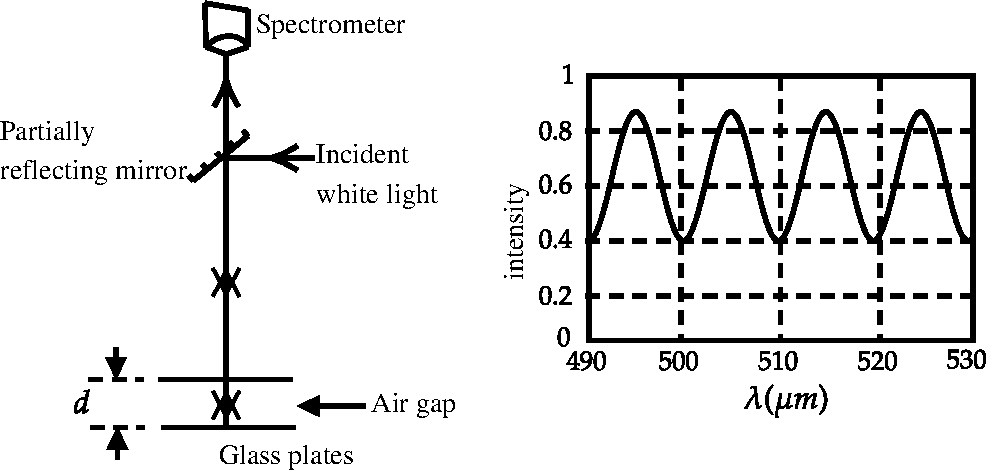
\includegraphics[height=4cm,width=8cm]{diagram-20211011(48)-crop}
	\end{figure}
	Assuming that the interference takes place only between light reflected by the bottom surface of the top plate and the top surface of bottom plate, the distance $d$ is closest to
	\exyear{NET DEC 2016}
\end{minipage}
\begin{tasks}(2)
	\task[\textbf{A.}] $12 \mu \mathrm{m}$
	\task[\textbf{B.}] $24 \mu m$
	\task[\textbf{C.}] $60 \mu m$
	\task[\textbf{D.}] $120 \mu \mathrm{m}$
\end{tasks}
\begin{answer}
	For constructive interference of reflected light, $2 d \cos \theta=\left(n+\frac{1}{2}\right) \lambda$.\\
	First maxima occurs at $\lambda=495 \mu m, \theta=0^{\circ}$ and $n=0 .$ Thus, $d=\frac{\lambda}{4}=\frac{495 \mu m}{4} \approx 120 \mu m$	\\
	The correct option \textbf{(d)}
\end{answer}
\begin{minipage}{\textwidth}
	\item The figure describes the arrangement of slits and screens in a Young's double slit experiment. The width of the slit in $S_{1}$ is $a$ and the slits in $S_{2}$ are of negligible width.
	
	If the wavelength of the light is $\lambda$, the value of $d$ for which the screen would be dark is
	\exyear{NET JUNE 2017}
	\begin{figure}[H]
		\centering
		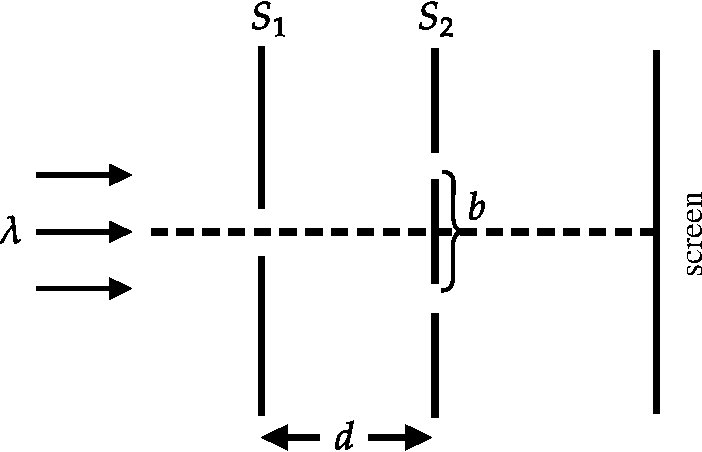
\includegraphics[height=4cm,width=6cm]{diagram-20211011(52)-crop}
	\end{figure}
\end{minipage}
\begin{tasks}(2)
	\task[\textbf{A.}] $b \sqrt{\left(\frac{a}{\lambda}\right)^{2}-1}$
	\task[\textbf{B.}]$\frac{b}{2} \sqrt{\left(\frac{a}{\lambda}\right)^{2}-1}$
	\task[\textbf{C.}]$\frac{a}{2}\left(\frac{b}{\lambda}\right)^{2}$
	\task[\textbf{D.}]$\frac{a b}{\lambda}$
\end{tasks}
\begin{answer}
	\begin{figure}[H]
		\centering
		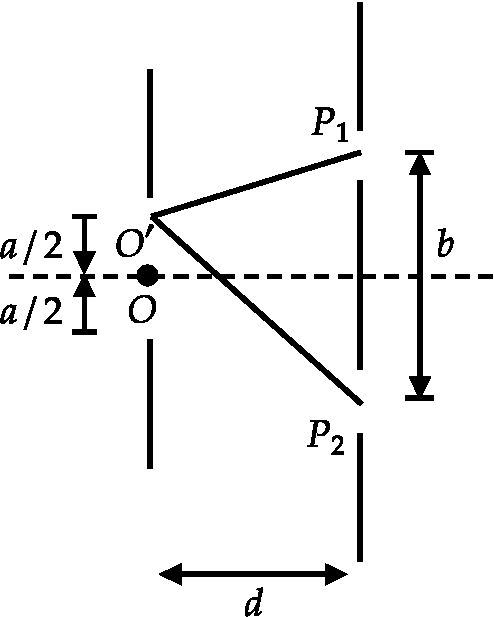
\includegraphics[height=5cm,width=5cm]{diagram-20211011(53)-crop}
	\end{figure}
	Solution: If the path difference $O^{\prime} p_{2}-O^{\prime} p_{1}=\frac{\lambda}{2}$
	The minima of the interference pattern produced by $O$ will fall on the maxima produced by $O^{\prime}$ Now
	$$
	\begin{aligned}
	&O^{\prime} P_{2}=\left[d^{2}+\left(\frac{b}{2}+\frac{a}{2}\right)^{2}\right]^{1 / 2} \approx d+\frac{1}{2 d}\left(\frac{b}{2}+\frac{a}{2}\right)^{2} \\
	&O^{\prime} P_{1}=\left[d^{2}+\left(\frac{b}{2}-\frac{a}{2}\right)^{2}\right]^{1 / 2} \approx d+\frac{1}{2 d}\left(\frac{b}{2}-\frac{a}{2}\right)^{2}
	\end{aligned}
	$$
	$$\begin{aligned}
	&\Rightarrow O^{\prime} P_{2}-O^{\prime} P_{1} \approx \frac{a b}{2 d} \quad(\because d>>b, a) \\
	&\text { Thus } \frac{\lambda}{2}=\frac{a b}{2 d} \Rightarrow d=\frac{a b}{\lambda}
	\end{aligned}$$
\end{answer}
\begin{minipage}{\textwidth}
	\item The following configuration of three identical narrow slits are illuminated by monochromatic light of wavelength $\lambda$ (as shown in the figure below). The intensity is measured at an angle $\theta$ (where $\theta$ is the angle with the incident beam) at a large distance from the slits. If $\delta=\frac{2 \pi d}{\lambda} \sin \theta$, the intensity is proportional to
	\exyear{NET JUNE 2018}
	\begin{figure}[H]
		\centering
		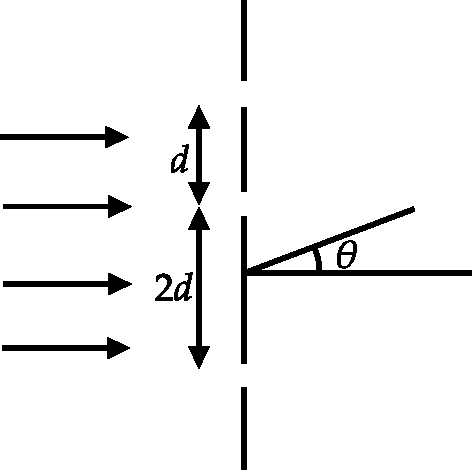
\includegraphics[height=3cm,width=5cm]{diagram-20211011(10)-crop}
	\end{figure}
\end{minipage}
\begin{tasks}(2)
	\task[\textbf{A.}] $2 \cos \delta+2 \cos 2 \delta$
	\task[\textbf{B.}]$3+\frac{1}{\delta^{2}} \sin ^{2} 3 \delta$
	\task[\textbf{C.}] $3+2 \cos \delta+2 \cos 2 \delta+2 \cos 3 \delta$
	\task[\textbf{D.}]$2+\frac{1}{\delta^{2}} \sin ^{2} 3 \delta$
\end{tasks}
\begin{answer}
	$$	\begin{aligned}
	\vec{E}_{1}=\vec{A} e^{i(\omega t)}, \vec{E}_{2}=\vec{A} e^{i \delta} e^{i \omega t}, \vec{E}_{3}=\vec{A} e^{i \delta_{1}} e^{i \omega t}=\vec{A} e^{3 i \delta} e^{i \omega t} \\
	&\because \delta=\frac{2 \pi}{\lambda} d \sin \theta, \delta_{1}=\frac{2 \pi}{\lambda}(3 d \sin \theta) \approx 3 \delta
	\end{aligned}$$
	$$\begin{aligned}
	&\vec{E}=\vec{E}_{1}+\vec{E}_{2}+\vec{E}_{3}=\vec{A}\left[1+e^{i \delta}+e^{3 i \delta}\right] e^{i \omega t} \\
	&\vec{E}^{*}=\vec{A}^{\prime}\left[1+e^{-i \delta}+e^{-3 i \delta}\right] e^{-i \omega t} \\
	&I=\vec{E} \cdot \vec{E}^{*}=A^{2}\left[1+e^{i \delta}+e^{3 i \delta}\right]\left[1+e^{-i \delta}+e^{-3 i \delta}\right] \\
	&I=A^{2}\left[3+2 \frac{e^{i \delta}+e^{-i \delta}}{2}+2 \frac{e^{i 2 \delta}+e^{-i 2 \delta}}{2}+2 \frac{e^{i 3 \delta}+e^{-i 3 \delta}}{2}\right] \\
	&I=A^{2}[3+2 \cos \delta+2 \cos 2 \delta+2 \cos 3 \delta]
	\end{aligned}$$
\end{answer}
\begin{minipage}{\textwidth}
	\item A monochromatic and linearly polarized light is used in a Young's double slit experiment.
	A linear polarizer, whose pass axis is at an angle $45^{\circ}$ to the polarization of the incident
	wave, is placed in front of one of the slits. If $I_{\max }$ and $I_{\min }$, respectively, denote the maximum and minimum intensities of the interference pattern on the screen, the visibility, defined as the ratio $\frac{I_{\max }-I_{\min }}{I_{\max }+I_{\min }}$, is
	\exyear{NET DEC 2018}
\end{minipage}
\begin{tasks}(2)
	\task[\textbf{A.}] $\frac{\sqrt{2}}{3}$
	\task[\textbf{B.}]$\frac{2}{3}$
	\task[\textbf{C.}]$\frac{2 \sqrt{2}}{3}$
	\task[\textbf{D.}]$\sqrt{\frac{2}{3}}$
\end{tasks}
\begin{answer}
	\begin{figure}[H]
		\centering
		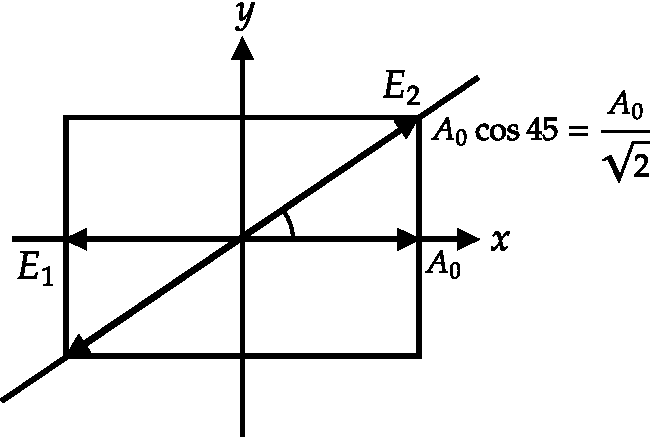
\includegraphics[height=4cm,width=5cm]{diagram-20211011(14)-crop}
	\end{figure}
	$$
	\begin{aligned}
	& \vec{E}_{1}=\hat{x} A_{0} e^{i \omega t} ; \quad \vec{E}_{2}=\frac{A_{0}}{\sqrt{2}} \frac{(\hat{x}+\hat{y})}{\sqrt{2}} e^{i \omega t+i \delta} \\
	&\qquad \begin{array}{l}
	I=\left(\vec{E}_{1}+\vec{E}_{2}\right) \cdot\left(\vec{E}_{1}^{*}+\vec{E}_{2}^{*}\right) \\
	\Rightarrow I=\left|\vec{E}_{1}\right|^{2}+\left|\vec{E}_{2}\right|^{2}+\vec{E}_{1} \cdot \vec{E}_{2}^{*}+\vec{E}_{2} \cdot \vec{E}_{1}^{*} \\
	=A_{0}^{2}+\frac{A_{0}^{2}}{4}+(1+1)+\frac{A_{0}^{2}}{2} e^{-i \delta}+\frac{A_{0}^{2}}{2} e^{i \delta} \\
	\Rightarrow I=A_{0}^{2}+\frac{A_{0}^{2}}{2}+\frac{A_{0}^{2}}{2} \frac{e^{i \delta}+e^{-i \delta}}{2}=\frac{3 A_{0}^{2}}{2}+A_{0}^{2} \cos \delta \\
	I_{\max }=\frac{5 A_{0}^{2}}{2}, I_{\min }=\frac{A_{0}^{2}}{2} \Rightarrow V=\frac{I_{\max }-I_{\min }}{I_{\max }+I_{\min }}=\frac{2}{3}
	\end{array}
	\end{aligned}$$	
\end{answer}
\end{enumerate}




















\newpage
\begin{abox}
	Practice set 2 solutions
	\end{abox}
\begin{enumerate}
\begin{minipage}{\textwidth}
	\item Interference fringes are seen at an observation plane $z=0$, by the superposition of two plane waves $A_{1} \exp \left[i\left(\vec{k}_{1} \cdot \vec{r}-\omega t\right)\right]$ and $A_{2} \exp \left[i\left(\vec{k}_{2} \cdot \vec{r}-\omega t\right)\right]$, where $A_{1}$ and $A_{2}$ are real amplitudes. The condition for interference maximum is
	\exyear{GATE 2013}
\end{minipage}
\begin{tasks}(2)
	\task[\textbf{A.}] $\left(\vec{k}_{1}-\vec{k}_{2}\right) \cdot \vec{r}=(2 m+1) \pi$
	\task[\textbf{B.}]$\left(\vec{k}_{1}-\vec{k}_{2}\right) \cdot \vec{r}=2 m \pi$
	\task[\textbf{C.}] $\left(\vec{k}_{1}+\vec{k}_{2}\right) \cdot \vec{r}=(2 m+1) \pi$
	\task[\textbf{D.}] $\left(\vec{k}_{1}+\vec{k}_{2}\right) \cdot \vec{r}=2 m \pi$
\end{tasks}
\begin{answer}
	The correct option is \textbf{(b)}
\end{answer}
\begin{minipage}{\textwidth}
	\item In an interference pattern formed by two coherent sources, the maximum and minimum intensities are $9 I_{0}$ and $I_{0}$ respectively. The intensities of the individual wave are
	\exyear{GATE 2014}
\end{minipage}
\begin{tasks}(2)
	\task[\textbf{A.}] $3 I_{0}$ and $I_{0}$ 
	\task[\textbf{B.}]$4 I_{0}$ and $I_{0}$
	\task[\textbf{C.}]$5 I_{0}$ and $4 I_{0}$
	\task[\textbf{D.}]$9 I_{0}$ and $I_{0}$
\end{tasks}
\begin{answer}
	$I_{\max }=\left(\sqrt{I_{1}}+\sqrt{I_{2}}\right)^{2}$ and $I_{\min }=\left(\sqrt{I_{1}}-\sqrt{I_{2}}\right)^{2}$\\
	$9 I_{0}=\left(\sqrt{I_{1}}+\sqrt{I_{2}}\right)^{2}$ and $I_{0}=\left(\sqrt{I_{1}}-\sqrt{I_{2}}\right)^{2} \Rightarrow I_{1}=4 I_{0}$ and $I_{2}=I_{0}$\\
	The correct option is \textbf{(b)}	
\end{answer}
\begin{minipage}{\textwidth}
	\item In a Young's double slit experiment using light, the apparatus has two slits of unequal widths. When only slit- 1 is open, the maximum observed intensity on the screen is $4 I_{0}$. When only slit-2 is open, the maximum observed intensity is $I_{0}$. When both the slits are open, an interference pattern appears on the screen. The ratio of the intensity of the principal maximum to that of the nearest minimum is
	\exyear{GATE 2015}
\end{minipage}
\begin{answer}
	$$ \frac{I_{\max }}{I_{\min }}=\frac{\left(\sqrt{I_{1}}+\sqrt{I_{2}}\right)^{2}}{\left(\sqrt{I_{1}}-\sqrt{I_{2}}\right)^{2}}=\frac{\left(\sqrt{4 I_{0}}+\sqrt{I_{0}}\right)^{2}}{\left(\sqrt{4 I_{0}}-\sqrt{I_{0}}\right)^{2}}=\frac{\left(2 \sqrt{I_{0}}+\sqrt{I_{0}}\right)^{2}}{\left(2 \sqrt{I_{0}}-\sqrt{I_{0}}\right)^{2}}=\frac{9 I_{0}}{I_{0}}=9$$	
\end{answer}
\end{enumerate}